\documentclass{standalone}

\usepackage{amssymb} % мат. символы
    \DeclareMathSymbol{\sm}{\mathbin}{AMSa}{"39} % короткий минус
    \newcommand{\mo}{\sm\!1}

\usepackage{bm}
    \newcommand{\bma}{{\bm{\alpha}}}
    \newcommand{\bmb}{{\bm{\beta}}}
    
\usepackage{tikz}
    \usetikzlibrary{arrows.meta}
    \usetikzlibrary{calc}
    
\tikzset{gdst/.style=
    {circle, draw=black!50, very thick, minimum height=1.2cm, inner sep=2pt, text centered, }, }

\begin{document}
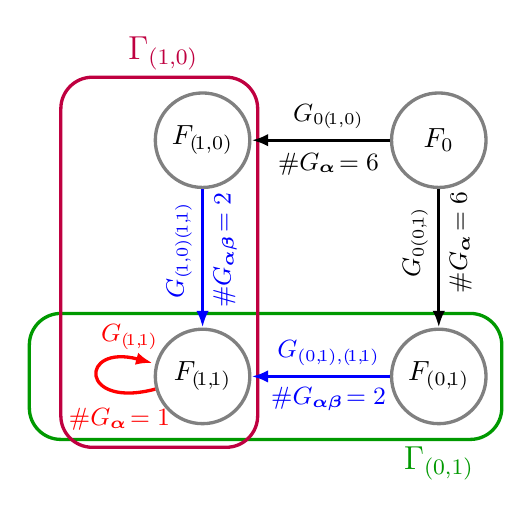
\begin{tikzpicture}
    \draw[green!60!black, very thick, rounded corners=4mm] (-2.2,-0.8)rectangle(3.8,0.8);
    \draw[purple, very thick, rounded corners=4mm] (-1.8,-0.9)rectangle(0.7,3.8);
    \node[gdst, shift={(0,0)}] (f1){$F_{(\mo,\mo)}$};
    \node[gdst, shift={(3,0)}] (f2){$F_{(0,\mo)}$};
    \node[gdst, shift={(0,3)}] (f4){$F_{(\mo,0)}$};
    \node[gdst, shift={(3,3)}] (f5){$F_{0}$};
    \path[->,>={Latex[length=6pt]}, very thick] 
        (f1)edge[loop left, red] 
                node[shift={(1.05,-0.55)}] {\small$\#G_{\bma}\!=1$}
                node[shift={(0.9,0.5)}] {\small$G_{(\mo,\mo)}$} (f1)
        (f2)edge[blue]
                node[below, shift={(0.1,0)}] {\small$\#G_{\bma\bmb}\!=2$}
                node[above, shift={(0.1,0)}] {\small$G_{(0,\mo),(\mo,\mo)}$} (f1)
        (f4)edge[blue] 
                node[below, rotate=90, shift={(0.1,0)}] {\small$\#G_{\bma\bmb}\!=2$}
                node[above, rotate=90, shift={(0.1,0)}] {\small$G_{(\mo,0)(\mo,\mo)}$} (f1)
        (f5)edge
                node[below, rotate=90, shift={(0.2,0)}] {\small$\#G_{\bma}\!=6$}
                node[above, rotate=90, shift={(0.2,0)}] {\small$G_{0(0,\mo)}$} (f2)
            edge
                node[shift={(0.1,-0.3)}] {\small$\#G_{\bma}\!=6$}
                node[shift={(0.1,0.3)}] {\small$G_{0(\mo,0)}$} (f4);
    \node[shift={(3,-1.1)}, green!60!black]{\large$\Gamma_{(0,\sm1)}$};
    \node[shift={(-.5,4.1)}, purple]{\large$\Gamma_{(\sm1,0)}$};
\end{tikzpicture}
\end{document}
% FSI_6x6_SG